%%!TEX root = diss.tex

\chapter{Calculation of the sediment flux}

\section{Introduction}

A relativity weak flow shearing a bed of sediment entrains individual particles into a state of motion controlled by turbulent forcing and intermittent collisions with other grains at rest on the bed, generating wide fluctuations in the sediment velocity \citep{Heyman2016,Fathel2015}.
Bed load particles move downstream until they are disentrained when they happen to encounter sufficiently sheltered divots on the bed surface to interrupt their motions \citep{Charru2004,Gordon1972}.
Eventually, the bed around them rearranges and destroys this shelter, or turbulent fluctuations overcome the shelter \citep{Celik2019,Valyrakis2014}, particles are once again entrained, and the cycle repeats.
Bed load transport is thus a kind of itinerant motion, characterized by alternation between fluctuating movements and rest.
This process has proven itself extremely challenging to describe mathematically, given the technicality of the stochastic physics required \citep{Pierce2020,Ancey2020}.

To date, descriptions of bed load transport have therefore simplified the problem in various ways to enable progress.
The foundational work is due to Einstein, who considering bed load motions as instantaneous, so he could describe bed load transport as an alternating sequence of ``steps" and rests having random length and duration \citep{Einstein1937}, in a pioneering application of the continuous time random walk \citep{Montroll1965}.
Einstein concluded that particles move downstream with a mean velocity $\bra u \ket = k_E l$, where $k_E$ is the rate at which an individual bed particle entrains into motion, and $l$ is the mean length of each downstream step.
Later, he applied these ideas to calculate the mean downstream flux of many particles \citep{Einstein1950}. Einstein reasoned that if the density of resting particles on the bed is $\rho_b$, the overall areal entrainment rate of particles can be written $E = \rho_b k_E$, so the mean downstream sediment flux can be expressed as $\bra q_s \ket = \rho_b \bra u \ket  = El $.

Many researchers have since refined Einstein's approach to provide more realistic descriptions of individual particle motions than Einstein's instantaneous step model.
One set of efforts has concentrated on particle motions only, calculating the downstream velocity distributions of moving particles using Langevin-type equations to describe turbulent flow and collision forces \citep{Ancey2014,Fan2014,Pierce2021}. These models do not yet include transitions between motion and rest. 
Another set of efforts has concentrated on including both motion and rest phases while promoting Einstein's instantaneous steps into finite periods of motion \citep{Lisle1998,Lajeunesse2017,Pierce2020b}, but due to mathematical challenges, these models characterize particle motions by a constant velocity, rather than the fluctuating velocities that real sediment particles exhibit.

Researchers have also refined stochastic formulations of the sediment flux beyond the description of the mean flux provided by Einstein \citep{Furbish2012}. Experiments demonstrate that the sediment flux exhibits wide fluctuations due to (1) variations in the number of moving particles and (2) variations in the velocities of moving particles \citep{Ancey2008, Ancey2014}.
As a result of these sediment tranport fluctuations, measurements of the mean sediment flux depend on the timescale over which they are collected \citep{Saletti2014,Dhont2019,Singh2009}, giving a scale-dependent character to the mean sediment flux.
To date, very few models have calculated the probability distribution of the bed load sediment flux, and among these, even fewer have described any observation-scale dependence of the sediment flux \citep{Ancey2019}.

This survey reveals two major issues in need of research attention. First, we do not yet have the capability to describe individual sediment trajectories through motion and rest including velocity fluctuations in the motion state; and second, we need more understanding of how to connect individual particle trajectories through motion and rest to the overall downstream sediment flux probability distribution and the dependence of the moments of this distribution on the observation time.
Here, we develop a new statistical physics-based formalism which addresses both of these problems by describing individual particle trajectories with a Langevin-type equation of motion. 
This stochastic equation includes alternation between motion and rest at random intervals, and the motion state includes stochastic forcing that ascribes fluctuating velocities to moving particles.
Using the probability distribution of particle position generated by this model, we construct a formalism to derive analytically the probability distribution of the sediment flux, and this distribution includes an explicit observation-scale dependence.
Below, we develop the new formalism in sec. \ref{sec:mod}, solve it in sec. \ref{sec:res}, and we discuss the implications of our results and future research ideas in secs. \ref{sec:disc} and \ref{sec:conc}.

\section{Model development \label{sec:mod}}
We consider an infinite one-dimensional domain populated with sediment particles on the surface of a sedimentary bed. We consider that the flow is weak enough that interactions among moving grains are very rare, although interactions between moving particles and the bed may be common. The flow is in constrast strong enough so that particles are in motion. 
We label the downstream coordinate as $x$, so that the downstream velocity of a moving particle is $\dot{x}$, and we describe all sediment particles as independent from one another, but governed by the same underlying dynamical equations, meaning we neglect any influence of sediment size or shape or spatial variations in the overlying fluid flow.

\subsection{Dynamical equation for bed load sediment transport}
From these assumptions, our first target is to write an equation of motion for the individual sediment particle encompassing two features. First, particles should alternate between motion and rest. The transition rate from rest to motion is called entrainment and occurs with probability per unit time (or rate) $k_E$, while the transition from motion to rest is called deposition and occurs with rate $k_D$. Second, particles in motion should move with mean velocity $V$ and some fluctuations around this velocity. 
The simplest equation of motion including these features is
\be \dot{x}(t) = [V + \sqrt{2D}\xi(t)]\eta(t).  \label{eq:langevin} \ee
Here $\xi(t)$ is a Gaussian white noise having zero mean and unit variance representing velocity fluctuations among moving particles, and $\eta(t)$ is a dichotomous noise which takes on values $\eta = 1$, representing motion, and $\eta=0$, representing rest. Here, $V$ is the mean particle velocity, and $D$ is a diffusivity [units $L^2/T$] of moving particles. The transition rate from $\eta=0$ to $\eta = 1$ is $k_E$, and the transition rate from $\eta=1$ to $\eta= 0$ is $k_D$. We write $k=k_E+k_D$ as a shorthand. 



%We will show later that $D=0$ reproduces the model of Lisle et al \citep{Lisle1998} for the sediment particle alternating between motion and rest with a constant velocity, while the further limit $k_D \rightarrow \infty$ as $V/k_D \rightarrow l$ reproduces the original theory of Einstein \citep{Einstein1937}.
\subsection{Derivation of the master equation for $P(x,t)$}
The solution of equation \ref{eq:langevin} for a given realization of the two noises $\eta(t)$ and $\xi(t)$ gives the trajectory of a single particle. Averaging over the ensemble of all such trajectories from different realizations of the noises will obtain the probability distribution $P(x,t)$ that a particle which started at position $x=0$ at time $t=0$ has travelled to position $x$ by time $t$. This distribution, by construction, will generalize earlier models which did not include velocity fluctuations among moving particles \citep{Lisle1998,Lajeunesse2017}.

We form the desired probability distribution of position as $ P(y,t) = \big\bra \delta(y-x(t))\big\ket_{\eta,\xi} $, where $x(t)$ is the formal solution of eq. \ref{eq:langevin} and the average is over both noises, but this symbolic equation is not yet useful as taking these averages directly is a challenging mathematical problem \citep{Hanggi1978}.
A simpler approach is to conduct the necessary averages in Fourier space. Integrating eq. 1, using its solution in the probability distribution, then Fourier transforming gives
\be \tilde{P}(g,t) = \Big\bra  \Big\bra \exp \Big[- i g \int_0^t du [V+\sqrt{2D}\xi(u)]\eta(u) \Big]\Big\ket_\eta \Big\ket_\xi.\ee
Taking time derivatives and conducting the averages using known characteristics of averages of exponentials of Gaussian white noise \citep{Gardiner1983,VanKampen1978} and the Furutsu-Norikov procedure for time derivatives of averages involving dichotomous noise \citep{Loginov1978}, in a method similar to \citep{Balakrishnan1993}, provides the Fourier-space master equation
\be \pt^2 \tilde{P}(g,t)  = (igV-g^2D-k)\pt  \tilde{P} + k_E (igV-g^2D) \tilde{P},\ee
and inverse Fourier transforming provides the master equation
\be (\pt^2 + V \px \pt + k_E V \px + k \pt - D \px^2 \pt - k_E D \px^2) P(x,t) = 0. \label{eq:master}\ee
This is a diffusion-like equation governing the probability distribution of position for individual particles as they transport downstream through a sequence of motions and rests, with the movement velocity being a random variable.
One can see in particular that taking an the entrainment rate $k_E$ very large, meaning that all particles are generally moving, implies an advection-diffusion equation $(\pt + V\px -D \px^2)P=0$ for the position, characteristic of a particle moving downstream with Gaussian velocity fluctuations. Otherwise, with $k_E$ of similar order as $k_D$, there is a finite probability that the particle is at rest, and the advection-diffusion process is often interrupted by deposition, giving rise to the additional terms in eq. \ref{eq:master}.
\section{Formalism for the downstream sediment flux}
Now we express the probability distribution of the sediment flux using the probability distribution of particle position $P(x,t)$ provided as the solution of equation \ref{eq:master}. We apply a modified version of the approach recently developed by Banerjee and coworkers for \citep{Banerjee2020}. The basic idea, as depicted in Figure 1, is that we distribute particles in all states of motion along a domain at random locations at $x<0$, then we calculate using $P(x,t)$ the rate of particle arrival to $x>0$ within the sampling time $T$.
\begin{figure}
	\centerline{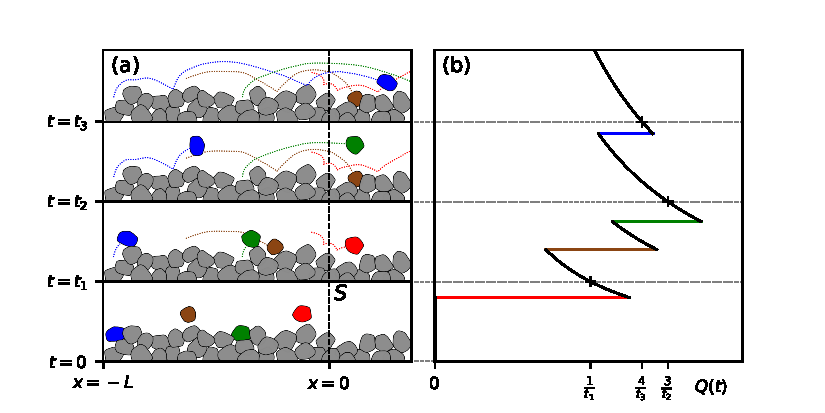
\includegraphics{./figures/ch2/figure1.pdf}}
	\caption{The left panel indicates the configuration for the flux. The particle trajectories within are calculated from equation \ref{eq:langevin}, demonstrating alternation between rest and motion with fluctuating velocity. Particles begin their transport with positions $-L\leq x \leq 0$ at $t=0$, and as depicted in the right panel, the flux is calculated as the number of particles $N_>(t)$ which lie to the right of $x=0$ at the observation time $t$, divided by $t$: $Q(t) = t^{-1}N_>(t)$. We calculate the probability distribution of $Q$ over all realizations of the trajectories and initial positions as $L\rightarrow \infty$}
	\label{fig:fig1}
\end{figure}

The rate of particles crossing the surface in an observation time $T$ is
\be Q(T) = \frac{1}{T}\sum_{i=1}^N \mathcal{I}_i(T). \ee
In this equation, $\mathcal{I}_i(T)$ is an indicator function which is $1$ whenever the $i$th particle has passed our control surface and $0$ otherwise. All particles which have not crossed the control surface (or which have crossed and then crossed back) contribute nothing to the flux. The probability distribution of the flux is then 
\be P(Q|T) = \Big \bra \delta\Big( Q - \frac{1}{T}\sum_{i=1}^N \mathcal{I}_i(T) \Big) \Big\ket. \ee
The average is over the initial conditions of each particle and the ensemble of trajectories for each particle.
Taking the Laplace transform over $Q$ (i.e. forming the characteristic function) obtains
\begin{align} \tilde{P}(s|T) &= \Bigg\bra \int_0^\infty dQ e^{-s Q}\delta\Big( Q - \frac{1}{T}\sum_{i=1}^N \mathcal{I}_i(T) \Big)\Bigg\ket \\
	&=  \Big\bra \exp\Big(\frac{s}{T}\sum_{i=1}^N \mathcal{I}_i(T)\Big)\Big\ket \\
	&=  \prod_{i=1}^N \Big\bra \exp\Big(-\frac{s}{T}\mathcal{I}_i(T)\Big)\Big\ket \\
	&= \prod_{i=1}^N \Big[1-\big(1-e^{-s/T}\big)\big\bra \mathcal{I}_i(T) \big\ket \Big] \end{align}
This progression relies on the independence of averages for each particle (so the average of a product is the product of averages) and the fact that  $ \mathcal{I}_i(T)$ is either $1$ or $0$ ($e^{ax} = 1-(1-e^a)x$ if $x=0,1$).
The average over initial conditions and possible trajectories for the $i$th particle can be written
\be \bra \mathcal{I}_i(t) \ket = \frac{1}{L}\int_L^0 dx' \int_0^\infty dx \mathcal{P}(x,t|x') =  \frac{1}{L}\int_0^L dx' \int_0^\infty dx \mathcal{P}(x,t|-x'), \ee
where $\mathcal{P}(x,t|x')$ is the probability density that the particle is found at position $x$ at time $t$ given it was initially at $x'$ at time $0$. This is the part of the flux that depends on the particle dynamics (ie instantenous velocities and entrainment/deposition characteristics).

Inserting (7) into (6) and taking the limit as $L\rightarrow \infty$ and $N \rightarrow \infty$ while the density of particles $\rho = N/L$ remains constant provides
\be \tilde{P}(s|T) = \lim_{N \rightarrow \infty} \Big(1 - \frac{1}{N}\big(1-e^{-s/T}\big)\mu(T) \Big)^N = \exp \Big[ -\big(1-e^{-s/T}\big)\mu(T) \Big].\ee
where $\mu(T) = \rho \int_0^\infty dx \int_0^\infty dx' \mathcal{P}(x,T|x')$ is a rate constant which encodes the particle dynamics. This expression is the characteristic function of a Poisson distribution.
Expanding in $e^{-s/T}$ and inverting the Laplace transform provides the distribution of the flux
\be P(Q|T) = \sum_{k=0}^\infty \frac{\mu(T)^k}{k!}e^{-\mu(T)}\delta(Q-\frac{k}{T}).\ee
This equation implies that the mean flux is $\bra Q \ket(T) = \int_0^\infty dQ Q P(Q|T) = \mu(T)/T$, and similarly the variance is $\sigma_Q^2(T) = \mu(T)/T^2$. The conclusion is that if the flux is considered as a time averaged number of particles crossing a control surface, the mean flux is always Poissonian no matter how particles move, provided they do not interact with one another.

\section{Results \label{sec:res}}
\subsection{Derivation of the position probability distribution and its moments}
\begin{figure}
	\centerline{\includegraphics{figures/ch2/figure2_slopeKey.pdf}}
	\caption{The left panel shows the probability distribution of position evolving through time. From the initial state, which is a mixture of moving and resting particles, the distribution splits at short times into contributions from Delta function-like stationary particles and Normal-like moving particles. The right panel demonstrates the resulting spreading characteristics of particles. This short-time splitting noted in the left panel gives rise to ballistic diffusion at short timescales, followed by normal diffusion, as exemplified by equation \ref{eq:var}.}
	\label{fig:fig1}
\end{figure}
\be P(x,0) = \delta(x) \ee
\be \pt P(x,0) = -\frac{Vk_E}{k}\delta'(x) \ee
These initial conditions come from the initial state
\be P(x,0) = \lim_{t\rightarrow 0 } \frac{k_E}{k} \delta(x-Vt) + \frac{k_D}{k}\delta(x).\ee

\be \bar{\tilde{P}}(g,s) = \frac{s + k + Dg^2 - i g V k_D/k}{s(s+k)+(Dg^2-igV)(s+k_E)}. \ee
\be \tilde{P}(x,s) = \frac{-D\px^2 + Vk_D/k\px + s + k}{VR(s+k_E)}\exp\Big[\frac{Vx}{2D} - \frac{V|x|}{2D}R \Big]. \label{eq:laplace}\ee
\be R = \sqrt{1 + \frac{4D}{V^2}\frac{s(s+k)}{s+k_E}}\ee
\begin{multline} P(x,t) = \big[-D\px^2 + Vk_D/k \px + k + \delta(t)+ \pt \big]\int_0^t \mathcal{I}_0\Big( 2 \sqrt{k_Ek_D u(t-u)}\Big) e^{-k_E(t-u)} \\ \times \sqrt{ \frac{1}{4\pi D u}} \exp\Big[-k_D u - \frac{(x-Vu)^2}{4Du}\Big] du \end{multline}
The mean is $ \bra x \ket = k_E V t/k$.
The variance is 
\be \sigma_x^2 = 2\Big[ \frac{k_EV^2 k_D}{k^3} + \frac{k_ED}{k}\Big]\Big( \frac{1}{k}e^{-kt} - \frac{1}{k} + t \Big) \label{eq:var}\ee
\subsection{Calculation of the flux}
\be \mu(t) = \rho \int_0^\infty dx_i \int_0^\infty dx P(x+x_i,t).\ee

Taking the Laplace transform,
\be \tilde{\mu}(s) = \rho \int_0^\infty dx_i \int_0^\infty dx \tilde{P}(x+x_i,s).\ee


\begin{multline} 
	\mu(t) = \rho \int_0^t \mathcal{I}_0\Big(2\sqrt{k_Ek_Du(t-u)}\Big)e^{-k_E(t-u)-k_D u} \\
	\times \Bigg[\sqrt{\frac{D}{\pi u}}\Big([\cev{\partial_t} + k]u-\frac{1}{2}\Big)e^{-V^2 u/4D} + \frac{V}{2}\Big([\cev{\partial_t} + k]u -\frac{k_D}{k}\Big) \erfc\Bigg(-\sqrt{\frac{V^2 u}{4D}}\Bigg)\Bigg] du.
\end{multline}
\subsection{Connection to earlier work}
\section{Discussion \label{sec:disc}}
\subsection{The role of stochasticity in landscape evolution}
\subsection{Methods to calculate the sediment flux}
\subsection{Outlook and future research}
\section{Conclusion \label{sec:conc}}
